\documentclass[tikz]{standalone}

\usepackage[T1]{fontenc}
\usepackage[english]{babel}

\begin{document}
    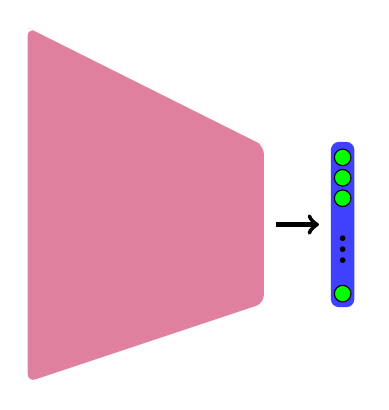
\begin{tikzpicture}
        \path[rounded corners=3pt, fill=purple!50] (2.5, 1) -- (5.5, -.5) -- (5.5, -2.5) -- (2.5, -3.5) -- (2.5, 1) -- (5.5, -.5);

        \path[rounded corners=3pt, fill=blue!75] (6.35, -.45) rectangle (6.65, -2.55);

        \node (top) at (6.5, -.5) {};
        \path (top) + (0, -1pt) node[anchor=north, circle, draw=black, fill=green, inner sep=0pt, text width=6pt] (first) {};
        \path (first.south) + (0, -1pt) node[anchor=north, circle, draw=black, fill=green, inner sep=0pt, text width=6pt] (second) {};
        \path (second.south) + (0, -1pt) node[anchor=north, circle, draw=black, fill=green, inner sep=0pt, text width=6pt] (third) {};
        \path (third.south) + (0, -1pt) node[anchor=north] (dots) {\Huge \(\vdots\)};
        \path (dots.south) + (0, -4pt) node[anchor=north, circle, draw=black, fill=green, inner sep=0pt, text width=6pt] (last) {};

        \path[->, ultra thick, draw=black] (5.65, -1.5) -- (6.2, -1.5);
    \end{tikzpicture}
\end{document}
